\documentclass{article}
\usepackage{graphics,html}
\title{Javascript API for Ravel 1.x}
\author{Ravelation Pty Ltd}
\begin{document}
\maketitle
\section{Getting Started}
Ravel is a C++ library compiled to Javascript via the Emscripten
compiler.

To insert a Ravel widget in your HTML document, create a
canvas element, then pass the canvas's ID to the factory function {\tt
  newRavel}. Finally, add some data describing the handles and you're
ready to go. For example, from the top level page of the Ravelation website.

\begin{verbatim}
<script type="text/javascript" src="examples/jsravel.js"></script>
<script type="text/javascript" src="examples/ravel.js"></script>
<canvas width="500" height="500" id="ravel"></canvas>
<script type="text/javascript" >
var ravel=newRavel("ravel");
ravel.addHandle("Year",["1990","1991","1992"]);
ravel.addHandle("Gender",["Male","Female"]);
ravel.addHandle("Country",["Australia","UK","USA"]);
ravel.redraw();
function onunload() {ravel.delete();}
</script>
\end{verbatim}

\begin{itemize}
\item {\em jsravel.js} is the compiled C++ Ravel library, which you must buy
  a license to use on your websites or applications.

\item {\em ravel.js} is some supporting native Javascript code, which
  provides UI bindings for the ravel widget, and some support for
  loading data from a MySQL database.

\item {\em newRavel} is a generator function for creating a Ravel
  object. It takes the HTML element id of a canvas element in the DOM.  
  Unfortunately, the embind library is somewhat limited in its support
  for subclassing C++ objects in Javascript, which is why you can't
  just have ``new Ravel'' in the code.

\item {\em Ravel::addHandle} adds a handle to the Ravel object, with axis name
  given by the first argument, and a list of slice labels given by the
  second argument.
  
\item {\em Ravel::redraw()} updates the image of the ravel on the
  screen. This is automatically called whenever the ravel state
  changes due mouse or keyboard action

\item {\em Ravel::delete()} Calls the C++ destructor for
  Ravel. Because Javascript has no finaliser concept that would allow
  this to be called when garbage collection runs, it is necessary
  to delete any created C++ objects when finished with, otherwise you
  may consume excessive amounts of memory.
\end{itemize}

\section{Ravel Terminology}

A ravel provides a way of manipulating $n$-dimensional datasets. Each
dimension is controlled by a {\em handle}, which looks like an
arrow. The dimensionality of the ravel's output data is called the
{\em rank}. Typical applications might have a rank 1 ravel (for
controlling plots or timeseries) or rank 2 (for controlling
spreadsheets or surface plots).

Handles may be {\em output handles}, which control the dimensions of
the output dataset, or other, non-output handles. Handles may
be swapped by rotating the handle, potentially turning an output
handle into a non-output handle and vice-versa. A non-output handle
will have a {\em slicer control}, which control which slice is output
by the ravel. The labels along a handle are known as {\em slice labels}.

When a handle is {\em collapsed} (by dragging the handle tip towards
the origin), the entire dataset is {\em reduced} along that dimension
by applying an arithmetic operation between the values. {\em Reduction
operations} include sum, product, average, standard deviation, minimum
and maximum.

\section{Ravel Classes}

\begin{latexonly}
\resizebox{\textwidth}{!}{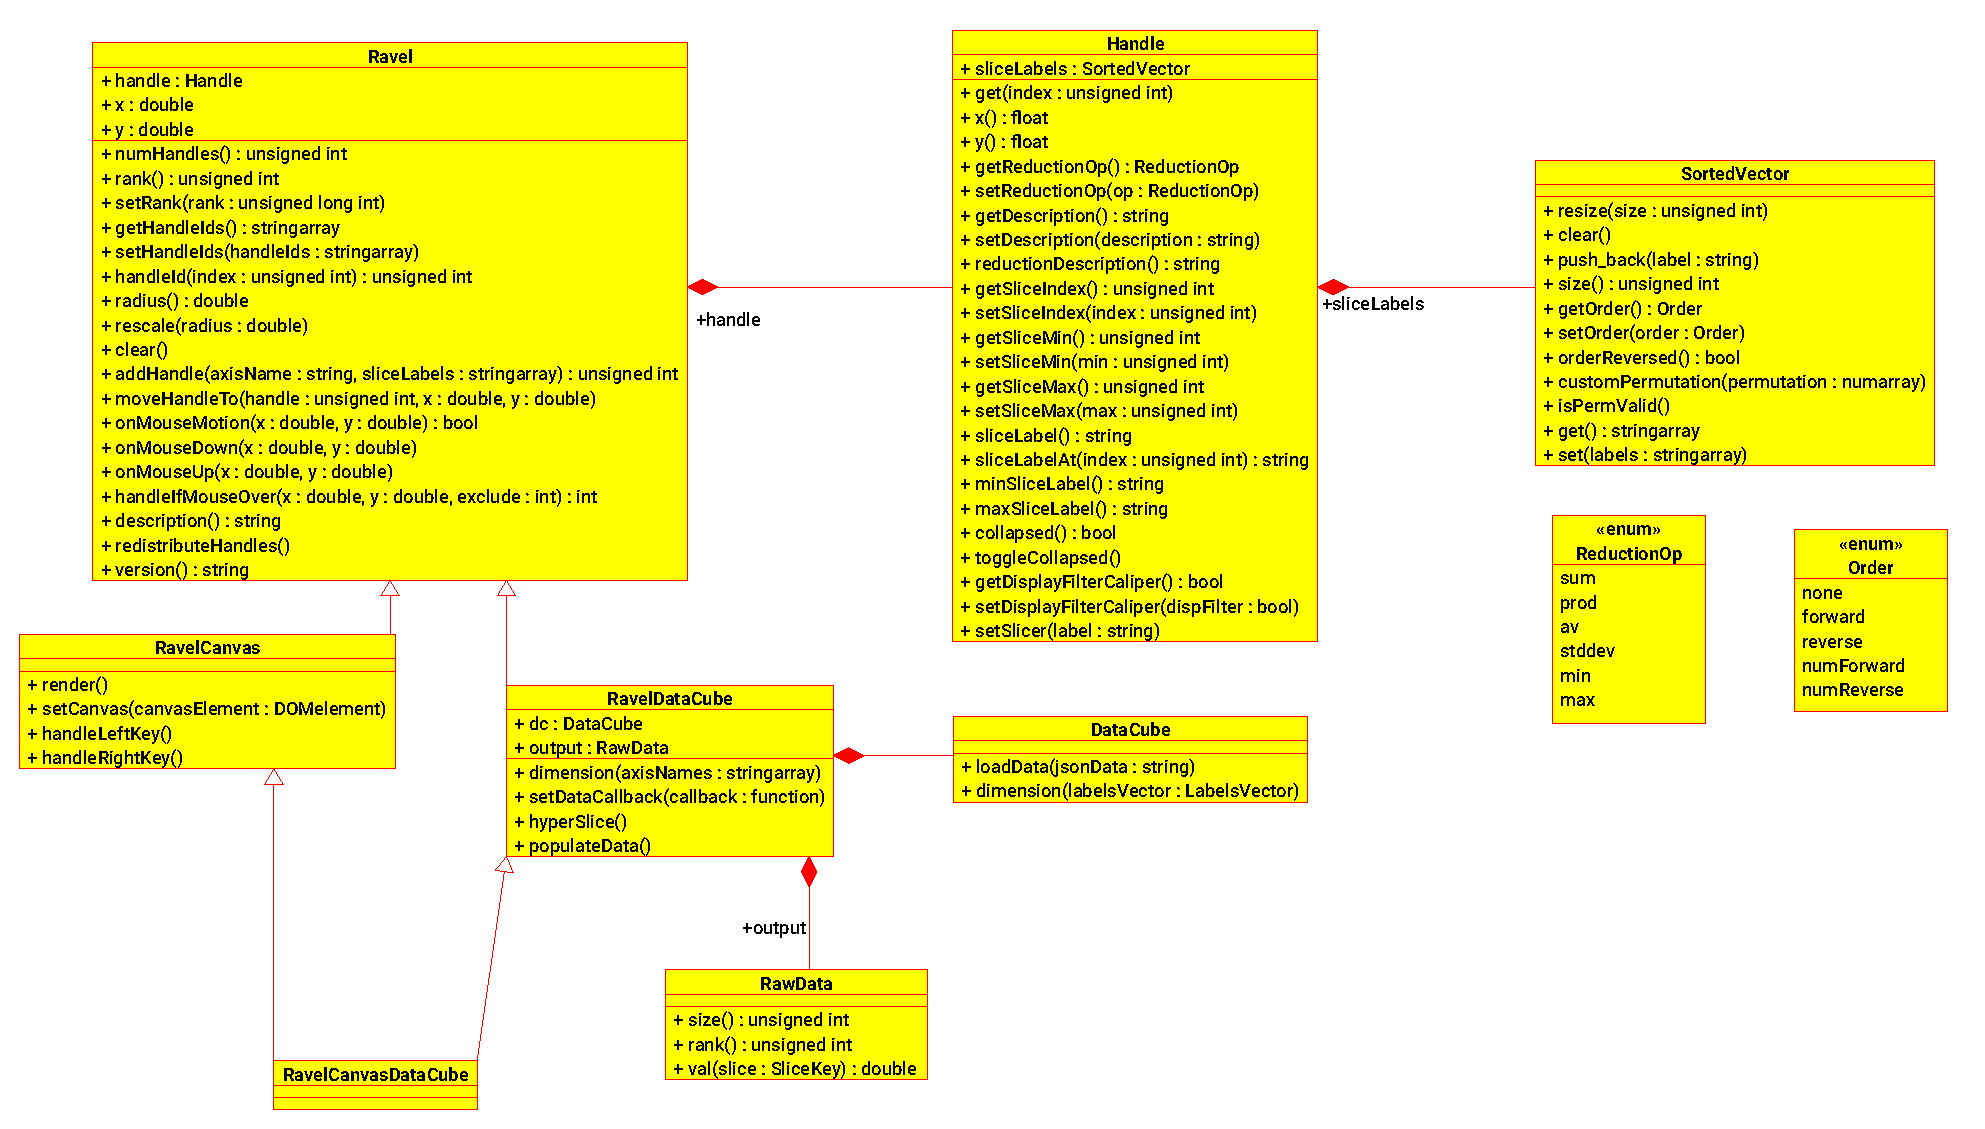
\includegraphics{javascriptAPI-UML.eps}}
\end{latexonly}

\begin{rawhtml}
  <iframe src="javascriptAPI-UML.svg" width="100\%" height="100\%" style="border:none"></iframe>
\end{rawhtml}

The Ravel library is written in C++, and compiled to Javascript via
the \htmladdnormallink{emscripten
compiler}{https://github.com/kripken/emscripten}. There are some
limitations with the Javascript interface generated by the current
emscripten implementation:
\begin{itemize}
\item C++ objects created by the system must be explicitly deleted by
  calling their \verb+delete+ method, otherwise a memory leak
  results. Unfortunately, Javascript has no concept of {\em finaliser}
  that is present in other garbage collected languages that would help
  here.
\item C++ methods returning complex data types will generate a new C++
  object, that needs to be deleted as well. Strings are an exception, in
  that they are simply converted into Javascript strings. In the following
  documentation, it will be noted if the returned object needs to be
  deleted.
\item C++ methods returning a reference do not return a reference
  object back to Javascript, but instead create a new C++ object that is
  a copy. Because of this, special reference members are added into
  containing objects that can be adjusted to point to desired
  object. Ravel::Handle is an example.
\item Method overloading is not supported in Javascript. Overloaded
  C++ methods must have different names in Javascript (even if the
  number of arguments differ). In particular, this means that
  getter/setter methods need distinct names, so we use the get/set{\em
    Attribute} convention here, even if the C++ equivalents are just the
  attribute name with setter/getter functionality distinguished by argument.
\item All C++ classes and other objects are created in the Module namespace.
\end{itemize}

\subsection{Module.Ravel}

\begin{description}
\item[Usage:] \verb+var ravel=new Module.Ravel+
  
\item[Properties:]\mbox{}
  \begin{description}
  \item[handle] of type Handle. A reference to one of the handles of the
    ravel. Initialise it to a particular ravel with
    \verb+ravel.handle.get(i)+, where \verb+i+ is the index of the desired
    handle. One consequence of this, and Javascript's object reference
    semantics is that you cannot refer simultaneously to two or more
    handles of the same ravel in the code.
  \item[x,y] The mouse coordinates of the centre of the Ravel. Used in
    methods that process mouse coordinates.
  \end{description}
  
\item[Methods:]\mbox{}
  \begin{description}
  \item[numHandles()] Returns the number of handles this ravel has.
    
  \item[rank()] returns the rank of the ravel. Equivalent to getHandleIds().length
  \item[setRank(rank)] sets the rank of the ravel. Equivalent to
    setHandleIds([0,1,...rank]);
  \item[getHandleIds()] returns an array of integer ids of the output handles
  \item[setHandleIds(array)] sets the array of integer ids of the output
    handles.
  \item[handleId(i)] returns the output handle index for the ith output
    handle. Equivalent to getHandleIds()[i].
  \item[version()] report the version of this ravel software
  \item[radius()] Returns the size of the ravel in pixels, from the origin
    to the handle tips.
  \item[rescale(radius)] Resize the ravel to have a radius {\tt radius}.
    
  \item[clear()] Removes all handles from the system.
    
  \item[moveHandleTo(handle, x, y)] moves the handle {\tt handle} to
    lie along the vector ({\tt x},{\tt y}). If the norm of ({\tt x},{\tt
      y}) is below the collapse threshold, the handle is collapsed. This is
    a somewhat low-level method, usually one should just use the {\tt
      onMouse}* event processing methods.
    
  \item[onMouseMotion(x,y)] Handle mouse motion. Handles are rendered
    differently when the mouse point is hovering over a
    handle. If the mouse button is pressed, then the handle is moved
    to the location of the mouse. Returns true if the ravel needs to be redrawn.
  \item[onMouseDown(x,y)] Handle mouse button press event.
  \item[onMouseUp(x,y)] Handle mouse button release event.
    
  \item[handleIfMouseOver(x,y,exclude)] Returns the index of a handle if
    the mouse is hovering over it. If the mouse is not hovering over any
    handle, then -1 is returned. If exclude is positive, then -1 is
    returned even if the mouse is hovering over the handle given by {\tt
      exclude}.

  \item[description()] returns descriptive text of the operation of the
    ravel (plain English for now)
    
  \item[redistributeHandles()] Rank 1 ravels place the output handle in
    the pointing east position, and the other handles distributed around
    the circle. Rank 2 ravels place the second output handle pointing
    south. The other handles are distributed evenly around the other 3
    quadrants. Current, ranks 3 or higher ranks are not supported.
    
  \end{description} 
\end{description} 

\subsection{Module.RavelCanvas}

A RavelCanvas combines a ravel with code to render the ravel to an
HTML canvas element. It subclasses Module.Ravel.

\begin{description}
\item[Usage:] \verb+var ravel=new Module.RavelCanvas+

\item[Methods:]\mbox{}
\begin{description}
\item[render()] render the Ravel to the canvas element
\item[setCanvas(canvas)] canvas is the canvas context of an actual DOM object, as returned
  by \verb+document.getElementById().getContext('2d')+ or similar.
\item[handleLeftKey()] called to adjust the slicer towards the origin
  on the handle the mouse is currently hovering over
\item[handleRightKey()] called to adjust the slicer away from the origin
  on the handle the mouse is currently hovering over
\item[onMouseLeave()] handle mouse leave events
\end{description}
\end{description}

The key handling methods are in this class, because Module.Ravel has
no concept of a selected handle.

\subsection{Module.DataCube}

A DataCube represents a complete dataset being manipulated by a
Ravel. It's not much use on its own, but rather needs to be coupled
with a Ravel.

\begin{description}
\item[Usage:] \verb+var ravel=new Module.DataCube+

\item[Methods:]\mbox{}
\begin{description}
\item[loadData(jsonData)] load the datacube from an array of data
  (passed as a JSON string). Interpretation of the data is by the
  parameters set in dimension
\item[dimension(labelsVector)] Labels vector is a javascript array of
  objects describing an axis handle:
\begin{verbatim}
{
  axis: "axis name",
  slice: ["sliceLabel1",..."sliceLabeln"]
} 
\end{verbatim}
\end{description}
\end{description}

\subsection{Module.RavelDataCube}

A RavelDataCube is a Ravel that has a DataCube object.

\begin{description}
\item[Usage:] \verb+var ravel=new Module.RavelDataCube+
  
\item[Properties:]\mbox{}
  \begin{description}
  \item[dc] The DataCube object
  \item[output] The output hyperslice of type RawData
  \end{description}
  
\item[Methods:]\mbox{}
  \begin{description}
  \item[dimension(axisNames)]  Specifies the dimensions of the datacube
    object. Only the axis names need to be supplied, as the sliceLabels
    are inferred from the Ravel's configuration.
  \item[hyperSlice()] Sets the output property to contain the output
    data of the ravel in its current state (data slice). 
  \item[setDataCallback(f)] Sets a callback function for the
    populateData() call. This is only useful for rank 2 ravels. f has
    signature
\begin{verbatim}
var f=function(idx,v) {var col=idx[0], row=idx[1];...}
\end{verbatim}
where idx is an array of indices along the output handles (0-based),
and v is the output value at that location. This function will only be
called if a value exists at that location. The above example shows
decoding a rank 2 ravel, which is currently all that is supported.
\item[populateArray()] Computes the hyperslice for a rank 2 ravel,
call the callback function for all output values.

  \end{description}
\end{description}

\subsection{Module.RavelCanvasDataCube}

Usage: \verb+var ravel=new Module.RavelCanvasDataCube+

A RavelCanvasDataCube is both a RavelCanvas and a RavelDataCube. It
doesn't introduce any new properties or methods.

\subsection{Module.RawData}

\begin{description}
\item[Usage:]\mbox{}
\begin{verbatim}
var slice=ravel.output;
ravel.hyperSlice();
\end{verbatim}

\item[Methods:]\mbox{}
  \begin{description}
  \item[size()] Total number of elements in the output
  \item[rank()] Rank of the data slice
  \item[val(key)] Returns the value at a particular location indexed
    by key. NaN is returned if no such value exists. key is a
    Javascript array of structs:
\begin{verbatim}
{
  axis: "axisName",
  slice: "slice label"
}
\end{verbatim}
  \end{description}
\end{description}  

\subsection{Module.Handle}
  
The Handle class represents the handles of the ravel, that allow the
axes to be manipulated. It is a reference class, so not something that
can be independently created, but rather set to refer to the different
handles of a ravel.

\begin{description}
\item[Usage:]\mbox{}
\begin{verbatim}
var handle=ravel.handle;
handle.get(i);
\end{verbatim}

\item[Properties:]\mbox{}
  \begin{description}
  \item[sliceLabels] A SortedVector of the slice labels along the handle.
  \end{description}
  
\item[Methods:]\mbox{}
  \begin{description}
  \item[get(i)] sets the handle to refer to handle i, which should be in
    the range 0..ravel.numHandles().
  \item[x(), y()] coordinates of the handle tip.
  \item[getReductionOp()] returns the reduction that is applied when the
    handle is collapsed. The returned value is an enum type called
    Module.ReductionOp. Values are represented by static properties of
    that class, eg Module.ReductionOp.sum, and can be used in comparison
    operators or in case labels of a switch statement.
  \item[setReductionOp(op)] Sets the reductionOp attribute. op is one of
    the values of the Module.ReductionOp enum.
  \item[getDescription()] returns the axis label of this handle
  \item[setDescription(axisName)] sets the axis label of this handle
  \item[reductionDescription()] if the handle is collapsed, returns an
English language description of the reduction operation - eg ``sum of
countries", otherwise is equivalent to getDescription().
\item[getSliceIndex()] returns the position along the axis where the
  slicer control is position.
\item[setSliceIndex(idx)] sets the position of the slicer control
\item[getSliceMin()] returns the index of the minimum slice, when
  filtering is in effect
\item[setSliceMin(idx)] sets the minimum slice index
\item[getSliceMin()] returns the index of the maximum slice, when
  filtering is in effect
\item[setSliceMin(idx)] sets the maximum slice index
\item[sliceLabel()] returns the label at the current slicer
  control. Equivalent to sliceLabelAt(getSliceIndex()).
\item[sliceLabelAt(idx)] returns the label at index idx, given the
  current sort order.
\item[minSliceLabel()] equivalent to sliceLabelAt(getSliceMin())
\item[maxSliceLabel()] equivalent to sliceLabelAt(getSliceMax())
\item[collapse()] return whether the handle is collapsed
\item[toggleCollapsed()] toggles the collapsed state of the handle
\item[getDisplayFilterCaliper()] returns whether filtering has been
  enabled or not.
\item[setDisplayFilterCaliper(filter)] enable or disable filtering
  depending on whether filter is true or false.
\item[setSlicer(label)] sets the slicer to the position where label is
  found. If label is not a sliceLabel, then nothing happens. If the
  slice labels are not unique, then the action is indeterminate
\item[mask()] returns an array of boolean values. If a mask[i] is
  true, then no data items corresponding to slice i exist in the
  data. 
  \end{description}
\end{description}

\subsection{Module.SortedVector}

A vector of strings that can be reordered

\begin{description}
\item[usage:] \verb+var labels=ravel.handle.sliceLabels;+
  
\item[methods:]\mbox{}
\begin{description}
\item[resize(newSize)] resizes the vector. If newSize>size(), then the
  new positions will have empty labels. So this method is more useful
  for trimming entries off the end of the list. The order attribute is
  preserved, however any custom permutation is lost.
\item[clear()] Clears the vector. Equivalent to resize(0).
\item[push\_back(label)] pushes a new label onto the vector. Ordering
  is preserved, as described under resize().
\item[size()] returns the number of labels
  
\item[getOrder()] The order attribute is an enum Module.Order with the
  following values:
\begin{description}
\item[Module.Order.none] The order is in the same order the labels
  were originally added to the vector, or in custom order if a custom
  permutation is applied.
\item[Module.Order.forward] The labels are in lexicographic order
\item[Module.Order.reverse] The labels are in reverse lexicographic order
\item[Module.Order.numForward] The labels are in numerical order. If two labels
  have equal numerical prefix, they are ordered lexicographically.
\item[Module.Order.numReverse] The labels are in reverse numerical
order.
\end{description}
\item[setOrder(order)] sets the order attribute
  
\item[customPermutation(perm)] Apply a custom permutation to the
  sorting order. This overrides the effects of the order attribute. {\tt
    perm} is an array of the integers 0..size() in some permuted order.
\item[isPermValid()] returns true if the applied customPermutation is
  a valid permutation.
\item[get()] returns a javascript array of labels
\item[set(labels)] sets the vector to the array of labels
\end{description} 
\end{description} 

\section{ravel.js}

Ravel.js is a utility wrapper of javascript code distributed with the
javascript Ravel widget that helps setting up a ravel and connecting
it to a database. It is open source, so may be useful as a source of
studying the Ravel API.

\begin{description}
  \item[newRavel(canvasId)] returns a newly constructed
    RavelCanvasDatacube attached to the HTML canvas element with id
    {\tt canvasId}. Mouse and keyboard event handlers are wired up.

    ravel.onRedraw() is called every time the ravel is rerendered,
    allowing the ravel output data to be collected and processed.
    
  \item[setTable(name, ravel)] populates the RavelCanvasDataCube {\tt
    ravel} from the table {\tt name} using AJAX. {\tt
    ravel.dataLoadHook()} is called once data has finished loading.
  \item[populateTableSelector(selectorId)] populates an HTML select
    element with a list of table available in the database.
    \item[buildDbQuery(table,ravel)] build the query part of an AJAX call
      to mySqlService.php that returns just the hyperslice represented
      by {\tt ravel}, against the database {\tt table}. 
\end{description}

\section{mySqlService.php}

mySqlService.php is an implementation of a webservice that implements
generating hyperslices for the MySQL database. It is used in the
online examples on the Ravelation website.

The dataset is assumed to have a simple structure. The database needs
to have a separate row for each data element. There are two reserved
column names, id\$, which is the primary key (if any), and value\$ which
is the column containing the values. There is a column for each
dimension of the hypercube, filled with the slice labels for each data
item. The full hypercube of data need not be present - any missing
data is filled with NaN on output.

\subsection{mySqlService API}

\begin{description}
  \item[/mySqlService.php/axes] return the list of tables in the
    database as a JSON array
  \item[/mySqlService.php/axes/{\em table}] returns the list of axes
    (column names) for {\em table} as a JSON array
  \item[/mySqlService.php/axes/{\em table}/{\em axis}] returns the
    list of slice labels for axis {\em axis} of table {\em table} as a
    JSON array.
  \item[/mySqlService.php/allData/{\em table}] returns the contents
    of {\em table} as a single JSON array of doubles. Missing data
    is replace by NaN.
  \item[/mySqlService.php/data/{\em table}?{\em axis1=spec}\&{\em
      axis2=spec}...] returns a hyperslice of the table's dataset. The
    specification of the query string parameters are:
    \begin{description}
      \item[{\em axisName}=slice({\em label})] dataset is sliced along
        {\em axisName} at the value {\em label}.
      \item[{\em axisName}=reduce({\em op})] perform a reduction along
        {\em axisName}, using op (sum, prod, av, stddev, min, max).
      \item[{\em axisName}=filter({\em min},{\em max})] only return
        values in between min and max slice labels.
    \end{description}
\end{description}


    
\end{document}
